
%
\documentclass[conference]{IEEEtran}
\IEEEoverridecommandlockouts

\makeatletter
\def\ps@headings{%
\def\@oddhead{\mbox{}\scriptsize\rightmark \hfil \thepage}%
\def\@evenhead{\scriptsize\thepage \hfil \leftmark\mbox{}}%
\def\@oddfoot{}%
\def\@evenfoot{}}
\makeatother

\pagestyle{headings}
\def\figwidth{0.4\textwidth}
\def\subfigwidth{0.35\textwidth}
\def\temptablewidth{0.47\textwidth}




% *** CITATION PACKAGES ***
%
\usepackage{cite}
\usepackage{url}
\usepackage{graphicx}
\usepackage[cmex10]{amsmath}
\usepackage{cite}
\usepackage{subfigure}
\usepackage{color}
\usepackage{bm}
\usepackage{multirow}
\usepackage{longtable}
\usepackage{supertabular}
\usepackage{algorithm}
\usepackage{algorithmic}


\usepackage{epstopdf}
%\usepackage{algpseudocode}



% correct bad hyphenation here
\hyphenation{op-tical net-works semi-conduc-tor}

% newCommands
\newtheorem{theorem}{THEOREM}
\newtheorem{definition}{Definition}
\newtheorem{lemma}{Lemma}
\def \OPT {\rm{OPT}}
\def \ALG {\rm{ALG}}
\def \slab {\rm{slab}}
\def \type {\rm{type}}
\def \Time {\rm{TIME}}
\def \Traffic {\rm{TRAFFIC}}

\newsavebox{\ieeealgbox}
\newenvironment{boxedalgorithmic}
  {\begin{lrbox}{\ieeealgbox}
   \begin{minipage}{\dimexpr\columnwidth-2\fboxsep-2\fboxrule}
   \begin{algorithmic}}
  {\end{algorithmic}
   \end{minipage}
   \end{lrbox}\noindent\fbox{\usebox{\ieeealgbox}}}


\begin{document}
%
% paper title
% can use linebreaks \\ within to get better formatting as desired
\title{A Novel On-line Association Algorithm in Multiple-AP Wireless LAN}


% author names and affiliations
% use a multiple column layout for up to three different
% affiliations

\author{\IEEEauthorblockN{Liang Sun, Lei Wang, Zhenquan Qin, Zhuxiu Yuan\thanks{Zhenquan Qin is the corresponding author in Dalian University of Technology.}}
	\IEEEauthorblockA{School of Software,\\
		Dalian University of Technology, China\\
		liang.sun@dlut.edu.cn, lei.wang@dlut.edu.cn, qzq@dlut.edu.cn, zhuxiu.yuan@gmail.com}}

%\author{\IEEEauthorblockN{Michael Shell}
%\IEEEauthorblockA{School of Electrical and\\Computer Engineering\\
%Georgia Institute of Technology\\
%Atlanta, Georgia 30332--0250\\
%Email: http://www.michaelshell.org/contact.html}
%\and
%\IEEEauthorblockN{Homer Simpson}
%\IEEEauthorblockA{Twentieth Century Fox\\
%Springfield, USA\\
%Email: homer@thesimpsons.com}
%\and
%\IEEEauthorblockN{James Kirk\\ and Montgomery Scott}
%\IEEEauthorblockA{Starfleet Academy\\
%San Francisco, California 96678-2391\\
%Telephone: (800) 555--1212\\
%Fax: (888) 555--1212}}

% conference papers do not typically use \thanks and this command
% is locked out in conference mode. If really needed, such as for
% the acknowledgment of grants, issue a \IEEEoverridecommandlockouts
% after \documentclass

% for over three affiliations, or if they all won't fit within the width
% of the page, use this alternative format:
%
%\author{\IEEEauthorblockN{Haibo Ni\IEEEauthorrefmark{1},
%Lei Wang\IEEEauthorrefmark{1},
%Zhuxiu Yuan\IEEEauthorrefmark{1},
%Zhenquan Qin\thanks{Zhenquan Qin is the corresponding author in Dalian University of Technology. Lei Shu is the corresponding author in Guangdong University of Petrochemical Technology.}\IEEEauthorrefmark{1},
%Lei Shu\IEEEauthorrefmark{3}
%Ming Zhu\IEEEauthorrefmark{1},
%Di Wu\IEEEauthorrefmark{1},
%Wenzhe Zhang\IEEEauthorrefmark{1},
%XunTeng Xu\IEEEauthorrefmark{2} and
%Yuxuan Kang\IEEEauthorrefmark{1}}
%\IEEEauthorblockA{\IEEEauthorrefmark{1}School of Software\\
%Dalian University of Technology,
%Dalian, China 116621\\ Email: aaron.nihaibo@gmail.com, lei.wang@dlut.edu.cn, Zhuxiu,Yuan@gmail.com, qzq@dlut.edu.com}
%\IEEEauthorblockA{\IEEEauthorrefmark{2}HP Labs, China\\
%Email: xunteng.xu@hp.com}}
%\IEEEauthorblockA{\IEEEauthorrefmark{3}Guangdong Petrochemical Equipment Fault Diagnosis Key Laboratory,\\
%Guangdong University of Petrochemical Technology,
%Guangdong, China\\
%Email: lei.shu@lab.gdupt.edu.cn}}





% use for special paper notices
%\IEEEspecialpapernotice{(Invited Paper)}




% make the title area
\maketitle


\begin{abstract}
%\boldmath
Nowadays, wireless LAN has become the most widely deployed technology in mobile devices for providing Internet access. Operators and service providers remarkably increase the density of wireless access points in order to provide their subscribers with better connectivity and user experience. As a result, WLAN users usually find themselves covered by multiple access points and have to decide which one to associate with.  In traditional implementations, most wireless stations would select the access point with the strongest signal, regardless of traffic load on that access point, which might result in heavy congestion and unfair load.

   In this paper, we propose a novel on-line association algorithm to deal with any sequence of STAs during a long-term time such as one day.  We present a theoretical analysis that the competitive ratio of our association algorithm is $1-1/e$.  We evaluate the performance of our algorithm through simulation and experiments. Simulation results show that our algorithm improves the overall WLAN throughput by up to 37\%, compared with the conventional RSSI-based approach. Our algorithm also performs better than SSF (Strongest Signal First) and LAB (Largest Available Bandwidth) in the experiments.
\end{abstract}
% IEEEtran.cls defaults to using nonbold math in the Abstract.
% This preserves the distinction between vectors and scalars. However,
% if the conference you are submitting to favors bold math in the abstract,
% then you can use LaTeX's standard command \boldmath at the very start
% of the abstract to achieve this. Many IEEE journals/conferences frown on
% math in the abstract anyway.

% no keywords

\begin{IEEEkeywords}
    On-line Algorithm, Competitive Ratio, Association Algorithms, Wireless LAN
  \end{IEEEkeywords}


% For peer review papers, you can put extra information on the cover
% page as needed:
% \ifCLASSOPTIONpeerreview
% \begin{center} \bfseries EDICS Category: 3-BBND \end{center}
% \fi
%
% For peerreview papers, this IEEEtran command inserts a page break and
% creates the second title. It will be ignored for other modes.




\section{Introduction}
% no \IEEEPARstart
 Wireless local area networks (WLANs) have become a popular technology for access to the Internet and enterprise networks. As operators and service providers increase WLAN access points (APs) in many public areas, such as shopping mall, library, etc., WLAN users nowadays have higher chances to receive more than one AP signal in one spot. A crucial problem for WLAN users is to determine which AP to associate with. If selecting an inappropriate AP, a user will experience bad service, or even degrade other users' throughput.

  In conventional implementations of WLANs, each station (STA) scans multiple wireless channels to detect the APs within the communication range, and chooses an AP that has the strongest received signal strength indicator (RSSI). Thus, it is expected that an STA associates with an AP that has the strongest signal. However, this association approach can lead to inefficient utilization of the wireless network resources. The most apparent disadvantage of the RSSI-based STA association approach is that RSSI does not provide any information about the current traffic load of the AP \cite{he2010design}. It has been well established that when there are multiple STAs connected to the same AP with different physical transmission rates, then the saturation throughput of all STAs is bounded by the slowest transmission rate. Therefore, even though there are other less loaded APs in the region, most STAs may associate with the same AP, and experience congestion\cite{xu2010designing}. Furthermore, the throughput of STAs that are already associated with an AP will be severely affected by the other associated STAs with higher traffic demand. Thus how to select an AP in a WLAN to guarantee high throughput and balance load for each STA is a challenging issue\cite{kim2010alpha}.

  Obviously, the association algorithm can be used to achieve different objectives.  For instance, it can be used to maximize the overall throughput of a system\cite{nassiri2008novel}, achieve the network-wide bandwidth allocation fairness among STAs\cite{bredel2009understanding}, and balance the load among APs.  These plausible objectives can be obtained by one or two of the following parameters: the bit rate served by APs and the utilization of APs.  Though these plausible objectives can be obtained by the two parameters by the periodical off-line optimal solutions, these are not desired feasible association algorithm which could be implemented in real-world situations.  Consequently, more feasible association algorithms could deal with a sequence of STAs and maximize the overall traffic of a system.

  To achieve these objectives, we present a feasible on-line association algorithm in the premise of the bandwidth guaranteeing for associated STAs.  The main contributions of this work are summarized as follows.
  \begin{enumerate}
    \item We have designed a centralized on-line AP association algorithm which could deal with any sequence of STAs under the fixed bandwidth allocation mechanism.
    \item We have given a theoretical analysis that the competitive ratio of our association algorithm is $1-1/e$ under the fixed bandwidth allocation mechanism.  If for every instance, the ratio of the traffic of an on-line algorithm to that of the best off-line algorithm is at least $x$, the competitive ratio of the on-line algorithm is said to be~$x$.
    \item We have extended the association algorithm to ``early-leaving'' STAs.  We have also proven that the analysis is still valid in this condition.
%    \item We have given a description of an feasible strictly QoS bandwidth allocation mechanism.
  \end{enumerate}

    The rest of the paper is organized as follows. In Section~\ref{sec:related_work}, we discuss the related work. In Section~\ref{sec:network_system}, we describe the system model considered in the paper. Section~\ref{sec:algorithm} gives the problem formulation of the AP association in WLANs and presents the algorithm, followed by Section~\ref{sec:analysis} which analyzes the proposed algorithm.  We report the simulation and experimental results in Section~\ref{sec:evaluation}, and discuss some implementing issues in Section~\ref{sec:discussions}.  Finally, we conclude the paper in Section~\ref{sec:conclusion}.
% You must have at least 2 lines in the paragraph with the drop letter
% (should never be an issue)


\section{related work}\label{sec:related_work}
  Association algorithms for WLANs have been intensely studied by both the research community and the industry.  Fairness and load balancing are two interrelated dimensions of the AP association problem.  However, some works only consider one factor while trying to design an association mechanism. Li \textit{et al.}~\cite{li2012ap} took the fairness into account and proposed two algorithms, named NLAO-PF and BPF, respectively. They formulated the problem as a non-linear programming model to achieve proportional fairness. Kim \textit{et al.}~\cite{kim2012distributed} developed a framework for user association in infrastructure-based wireless networks, encompassing several different user association policies, collectively denoted $\alpha$-optimal user association. They also proposed an iterative distributed user association policy that adapted to spatial traffic loads and converged to a globally optimal allocation.

  Game theory is usually used to model the association control in wireless LANs since the association between an STA and an AP is affected by the behavior of other STAs and APs.  Yen \textit{et al.}~\cite{Yen:2011} modeled AP selection under the framework of game theory, where the goal of each STA was to maximize the achievable throughput, by considering both the number of STAs which associated with the same AP and the set of link rates these STAs possessed.  Keranidis \textit{et al.}~\cite{Keranidis:2011} made the AP selection for each STA in a distributed way to maximize total throughput of each STA, which was defined to be the sum of the throughput on the uplink and the downlink. Papaoulakis \textit{et al.}~\cite{Papaoulakis:2008} proposed an AP selection mechanism which the selection criterion was not limited to RSSI, but also to the traffic of the AP.  And it reconstructed a formula of the sum of the two factors as the new criterion.  Unfortunately, the paper did not give any convincing evidence about the advantages of his new criterion.



  None of the works mentioned above jointly considered the two interrelated dimensions in wireless LANs. Le \textit{et al.}~\cite{le2012maximizing} proposed a distributed algorithm where each STA selected an appropriate contention window size to fairly share the channel occupancy time while maximizing the aggregated throughput of the network.  Throughput based max-min fairness suffered from low network throughput in multi-rate wireless LANs~\cite{Bejerano:2004}.  To balance aggregate throughput while serving the STAs in a fair manner, Li \textit{et al.}~\cite{Li:2008} considered the proportional fairness over multi-rate wireless LANs, and proposed two approximation algorithms for periodical off-line optimization.  Proportional fairness, on the other hand, could effectively investigate the tradeoff between fairness and network throughput.  Bejerano \textit{et al.} presented an efficient solution to determine the STA-AP association with max-min fair bandwidth allocation~\cite{Bejerano:2004}, by leveraging the strong correlation between fairness and load balancing.

  Xie \textit{et al.}~\cite{Lei:2009} formulated the problem of AP association control over vehicular networks as a convex programming in the off-line setting, and presented a dynamic weight-based on-line algorithm to achieve proportional fairness.  Apparently, most of the on-line algorithms mentioned above need to run periodically, and they were an off-line algorithm at a time.

  Association algorithms in heterogeneous networks also become popular in recent years, Gong \textit{et al.}~\cite{gong2012ap} and Li \textit{et al.}~\cite{li2012optimal} proposed AP association methods in the heterogeneous network, considering fairness among STAs and load balancing. Besides, \cite{gong2012ap} also considered influence among different 802.11 protocols and the frame aggregation mechanism in 802.11n.

  Here we discuss a completely on-line algorithm with no need to run again when an STA is arriving or leaving.  Actually, it is difficult to give consideration to the two interrelated dimensions at the same time.  And there are many mechanisms to guarantee the quality of bandwidth allocated to the STAs~\cite{Ni:2004}.  Therefore, when we design an on-line association algorithm which could guarantee the quality of bandwidth of the associated STAs, we just consider the AP selection and the load balancing issues.

  Mehta \textit{et al.}~\cite{Mehta:2007} provided a simple framework to design a trade-off function between two factors in the on-line algorithm in.  The paper proposed an on-line algorithm with competitive ratio $1-1/e$ to solve the AdWords problem among the Internet search engine companies.  This paper introduced a new technique called \textit{a tradeoff-revealing family of LP's}, and outlined how to derive the correct tradeoff function.  Furthermore, the paper provided a method to deal with a more challenging situation that the bids of advertisers are arbitrary.  Based on the solution of the paper, we find that the capacity of each AP is limited, and the arrival and demand of the STAs are arbitrary. Therefore, we will apply this method to deal with the on-line case of our problem.


  \section{Network and System Description}\label{sec:network_system}
  \subsection{Network Model}
  We consider an IEEE 802.11e based WLAN that comprises a large number of APs.  Let $A$ denote the set of APs and let $N$ denote their quantity, i.e., $N=|A|$.  All APs are attached to a controller, which makes the decision of which AP an STA should associate with.  Each AP $a\in A$ has a theoretical traffic of $C_a$.  Each AP has a limited transmission range and it can only serve STAs that reside in its service range.

  We use $S$ to denote the set of mobile STAs that have resided in the network range during a long-term time $T$.  Our association algorithm is designed for the network in which STAs could arrive or depart freely. To the best of our knowledge, the network is regarded as stable when the time is measured in terms of tens of seconds.  Therefore, we focus on a long-term time such as one day as the running time of the algorithm.  Each STA is associated with a single AP to obtain service over a wireless channel.  Because we don't take infrastructure into consideration, for STA $s\in S$ and AP $a\in A$, we use the maximal bit rate between STA and AP as the total bandwidth of the AP. In this paper, we first consider STAs with specified required bandwidth $b_s$ and  time $t_s$.  APs will try to allocate the demanded bandwidth to its associated STAs, and STAs consume all bandwidth allocated to them and always have traffic to send or receive in their demanded time.  Furthermore, we consider a general case where STAs can leave before their demanded time is used up.

  \subsection{System Description}
  We develop a centralized on-line association mechanism that determines the appropriate STA-AP associations to maximize the network traffic in a long-term time.  Assuming each STA runs one session at one time, and specifies its required bandwidth in its demanded time.  Therefore, we regard each STA as a sequence of discontinuous STAs with a session which specifies a required bandwidth and demanded time.


  We now discuss the main implementation aspects of an association control system. First, the system requires the relevant information of the session on each STA, such as the bandwidth and time demand of the session, the maximal bit rate that it experiences from each AP.  Second, it needs an algorithm to determine the appropriate STA-AP association.  Third, it needs a mechanism to enforce these decisions, including association, handover without user interference, and denial of service.  In this study, we do not address the issue of providing the quality of bandwidth for STAs associated with a given AP.  We assume that such a mechanism is deployed at each AP, for instance, by using the emerging IEEE 802.11e extension~\cite{Ni:2004} or any fair bandwidth allocation, and we build our association algorithm on top of it.

  We observe that the required information, mainly the demanded bandwidth and time of the STAs and the maximal bit rate between STAs and APs, are not available.  The exact bandwidth and time demand decided by the session cannot be obtained by the STA before it runs.  One feasible scheme is that the STA obtains the information from the the application layer, and sends them to the AP as the requirements by some mechanism such as the web communication.  As for the maximal bit rate, an AP maintains the bit rate information only for the STAs who are currently associated with it.  We modify the beacon frame sent by nearby APs to measure the maximal bit rate that the STA can get from them.  All information will be reported to the the controller to make association decisions.

  \section{Algorithm Design}\label{sec:algorithm}
  This section, we focus on the network scenario that each STA runs only one session which specifies a demanded bandwidth in its demanded time at one time.  When an STA starts a new session, it reports its bandwidth demand and time demand to the APs by the controller.  The AP provides the new-coming STA with its demanded bandwidth, and allocates the remaining available bandwidth if its available bandwidth does not satisfy the STA's request.


  \subsection{Problem Definition}
  The AP association problem is the following:  There are $N$ APs, each with theoretical traffic $C_a$.  $S$ is a set of mobile STAs.  Each AP $a$ has the same total bandwidth $b_a$ for STA $s\in S$ without concerning about the relative position between them and the interference.  A sequence $s_1,s_2,\ldots,s_n$ of STAs $s_i\in S$ arrive on-line during $T$, and each STA $s_i$ must specify required bandwidth $b_{s_i}$ and time demand $t_{s_i}$ according to its current session. The objective is to maximize the overall traffic of system at the end of $T$ while respecting the quality of bandwidth of STAs. The notations and definitions to be used as summarized in Table~\ref{tb:notation}.
\begin{table}[!ht]
  \centering
  \caption{{\scshape Notations}}\label{tb:notation}
    \begin{tabular}{|c|p{6cm}|}
    \hline
    {\bf Symbol}& \hfil{\bf Semantics}\hfil \\
    \hline
    $A$ & The set of all access points \\
    \hline
    $S_a$ & The set of STAs which are associated with AP $s$\\
    \hline
    $S$ & The set of all STAs \\
    \hline
    $A_s$ & The set of candidate access points of STA $s$ \\
    \hline
    $C_a$ & The theoretical traffic of AP $a$ \\
    \hline
    $b_s$ & The demanded bandwidth of STA $s$\\
    \hline
    $b'_s$ & The actual allocated bandwidth of STA $s$\\
    \hline
    $t_s$ & The demanded time of STA $s$\\
    \hline
    $b_a$ & The total bandwidth of AP $a$\\
    \hline
    $\psi(a)$ & The trade\-off function on AP $s$\\
    \hline
    $N$ & The number of APs in the network\\
    \hline
    $n$ & The number of STAs which have associated with APs\\
    \hline
    $t_s$ & The time a new STA $s$ arrives\\
    \hline
    $T$ & The running time of the association algorithm\\
    \hline
    \end{tabular}
  \end{table}

  \subsection{Algorithm}
 \begin{figure}[!ht]
    \centering
    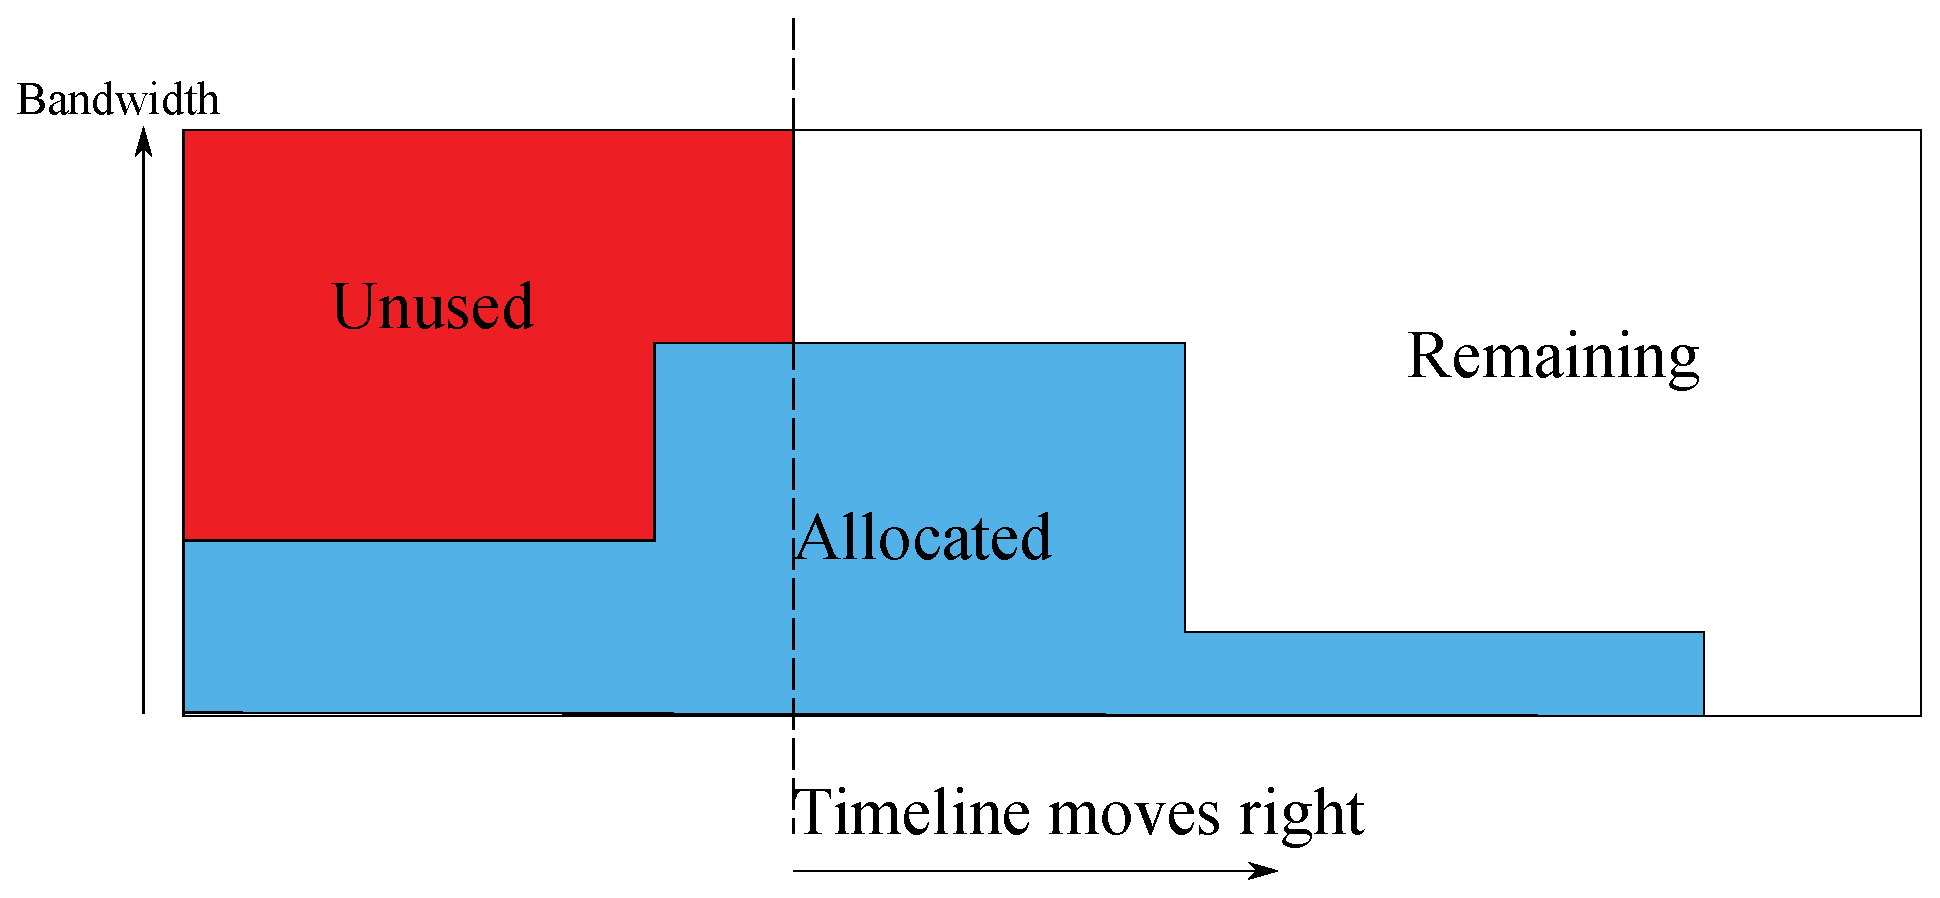
\includegraphics[width=\figwidth]{Three_parts.eps}\\
    \caption{The three parts of the theoretical traffic}\label{fig:Three_parts}
  \end{figure}

  \subsubsection{Difference With Generalized On-line Matching}
  When a new STA $s$ arrives at time $t_s$, we can divide the theoretical traffic into three parts in our association algorithm, the unused traffic before $t_s$, the allocated traffic and the remaining traffic after $t_s$ as shown in Fig. \ref{fig:Three_parts}. This is different from that of \cite{Mehta:2007} which has only used and remaining budget. So the theoretical analysis based on the AdWords model will be incorrect. In our opinion, letting the unused part be small enough can be a reasonable solution to  adapt to the AdWords model. In order to achieve this, we define the ``budget'' for an AP as the theoretical traffic during a specified amount of time(``budget time''). We also suppose the amount of budget is the same for every AP, and call this a \emph{budget window}. As our algorithm can only be valid during a short period of time at the beginning of budget window, we make the algorithm restart whenever the time-line reaches a specified short period(say, $1/k^2$ of ``budget time'') within budget window. Every time the algorithm restarts, the beginning of budget window ``jumps'' to the position of time-line. This way, as the area before time-line is always small enough compared to the budget window, we can simply ignore any unused traffic.

  Another difference between our model and the one in \cite{Mehta:2007} is that, besides the limit of budget, the STAs can't get more bandwidth than the available bandwidth the AP has. That is, the size of bid is limited. But we believe that this limit doesn't influence our algorithm and analysis due to the gernerality of the original model of on-line matching.

  \subsubsection{Algorithm}
  Now we will present our association algorithm when an STA $s$ arrives as shown in Algorithm~\ref{al:ap_association_algorithm}.  First, we define a trade-off function $\psi(x)$ of an AP as following:

  \begin{displaymath}
    \psi(x) = 1-e^{-(1-x)}.
  \end{displaymath}

  where $x$ will be substituted with the ratio of allocated traffic within the total traffic of the AP's budget window. To make it clear, the allocated traffic is the traffic that this AP has used to communicate with its associated STAs, plus that which it has planned to use with its associated STAs in the future. And the total traffic of the AP's budget window is the size of the budget window. So on the other side, the ratio is related to the \emph{free} traffic which this AP can allocate to upcoming STAs.

  It's easy to see that this function is monotonically decreasing as $x$, the ratio, increases.

  It's also convenient to discretize the traffic into $k$ equal parts, and we call each part a \emph{slab}, so each slab contains $\frac{1}{k}$ of the total traffic in budget window. The AP allocates from lower slabs first, and when lower slabs are emptied, higher slabs will be used. The slab which the AP is currently allocating traffic from is called an \emph{active} slab. We number each slab from $1$(lowest slab) to $k$(highest slab), and the active slab is $slab(i)$. Then we will get another form of the $\psi$ function:
  \begin{displaymath}
    \psi_k(i) = 1-e^{-(1-i/k)}.
  \end{displaymath}

   When an STA $s$ arrives, our algorithm runs, and chooses a proper AP for it. The STA $s$ must notify the centralized AP controller its demanded bandwidth and time. Then each AP makes a bid to this STA. The bid is in the unit of traffic, that is, the bid equals the amount of traffic the AP can allocate. Of course, not all AP can satisfy the bandwidth demand of $s$, as the available bandwidth of an AP might be smaller than it (i.e., $b_a-\sum_{s \in S_a}{b'_s} < b_s$). In this case, the AP bid with traffic smaller than $b_s \times t_s$. If this AP gets associated, from the next moment until an STA leaves, its bandwidth will be fully utilized.Formally, this would be: ($b'_s$ is the actual bandwidth allocated to the STA.)
  \begin{displaymath}
    b'_s = \begin{cases}
      b_s & b_a-\sum_{s \in S_a}{b'_s} \ge b_s; \\
      b_a-\sum_{s \in S_a}{b'_s} & \text{otherwise.}
    \end{cases}
  \end{displaymath}


    \begin{algorithm}[htb]
    \caption{\textsc{The AP-association algorithm}}\label{al:ap_association_algorithm}
    \begin{algorithmic}[1]
        \REQUIRE bandwidth and time demand of STA $s$, represented by
        $b_s$ and $t_s$
        respectively.
        \ENSURE $max\_priority\_ap$ of STA $s$
        \STATE $max\_priority \leftarrow -1$
        \FOR{$a$ in all APs}
        \STATE{$bid \leftarrow b'_s \times t_s$}
        \IF{$max\_priority < bid \times \psi_k(slab(i))$}
        \STATE{$max\_priority \leftarrow bid\times \psi_k(slab(i))$}
        \STATE{$max\_priority\_ap \leftarrow a$}
        \ENDIF
        \ENDFOR
        \STATE $max\_priority\_ap$ is the chosen AP for STA $s$.
    \end{algorithmic}
  \end{algorithm}



  \section{Theoretical Analysis}\label{sec:analysis}
  In this section we analyze the performance of our algorithm in the special case when all bids made by the candidate APs are equal.  Then the association algorithm can be simplified to a new  algorithm which is just based on the available traffic of the APs. For convenience, we call the new simplified algorithm as \textsc{Simplified-Association} algorithm as shown in Algorithm~\ref{al:simplified_association_algorithm}.

    \begin{algorithm}[htb]
    \caption{\textsc{The Simplified-association algorithm}}\label{al:simplified_association_algorithm}
    \begin{algorithmic}[1]
        \REQUIRE bandwidth and time demand of STA $s$, represented by
        $b_s$ and $t_s$
        respectively.
        \ENSURE $max\_priority\_ap$ of STA $s$
        \STATE $max\_priority \leftarrow -1$
        \FOR{$a$ in all APs}
        \IF{$max\_priority < \psi_k(slab(i))$}
        \STATE{$max\_priority \leftarrow \psi_k(slab(i))$}
        \STATE{$max\_priority\_ap \leftarrow a$}
        \ENDIF
        \ENDFOR
        \STATE $max\_priority\_ap$ is the chosen AP for STA $s$.
    \end{algorithmic}
  \end{algorithm}

  \subsection{Analyzing BALANCE using a Factor-Revealing LP}
  We wish to give a lower bound of the total traffic achieved  by {\scshape Simplified-Association Algorithm}.  Let us define the {\itshape type} of AP in a period according to the fraction of traffic served by that AP at the end of the algorithm {\scshape Simplified-Association Algorithm}: say that the AP in some period is of type $j$ if the fraction of its theoretical traffic spent at the end of the algorithm lies in the range $((j-1)/k,j/k)$,  By convention an AP in some period who spends none of his budget is assigned type 1.

  \begin{lemma}\label{le:type_slab}
    In some period, if OPT associates STA $s$ with AP $a$ of type $j\leq k-1$, then {\scshape Simplified-Association Algorithm} lays all demanded traffic of $s$ in some slab $i$ such that $i\leq j$.
  \end{lemma}

  The lemma follows immediately from the criterion used by {\scshape Simplified-Association Algorithm} for associating STAs with APs: $A$ has type $j\leq k-1$ and therefore transmits at most $j/k$ fraction of his theoretical traffic at the end of {\scshape Simplified-Association Algorithm}.  It follows that when STA $s$ arrives at the beginning of some period, $A$ is available to {\scshape Simplified-Association Algorithm} for associating with $s$,  and therefore $A$ must associate $s$ with some AP who has transmitted at most $j/k$ fraction of his total traffic in this period $s$.

  For simplicity we will assume that the AP in each period of type $i$ transmit exactly $i/k$ fraction of their theoretical traffic, that the amount of traffic pieces of each STA do not straddle slabs.  The second one is justified by fact the traffic piece is small compared to the traffic in each period (e.g. taking the piece to be smaller than $\frac{1}{k^2}$ of the traffic of each period).  The total error resulting from this simplification is at most $\frac{(2n-1)N}{k}$ and is negligible, once we take $k$ to be large enough.  Now, for $i=1,2,\ldots,k-1$, let $x_i$ be the number of periods for all APs of $\type(i)$.  Let $\beta_i$ denote the total traffic transmitted by the AP in each period from slab $i$ in \textsc{Balance}.  It is easy to see (Fig~\ref{fig:analysis_amount}) that $\beta_1=(2n-1)N/k$, and for $2\leq i\leq k$, $\beta_i=\frac{(2n-1)N}{k}-(x_1+\ldots+x_{i_1})/k$.
  \begin{figure}[!ht]
    \centering
    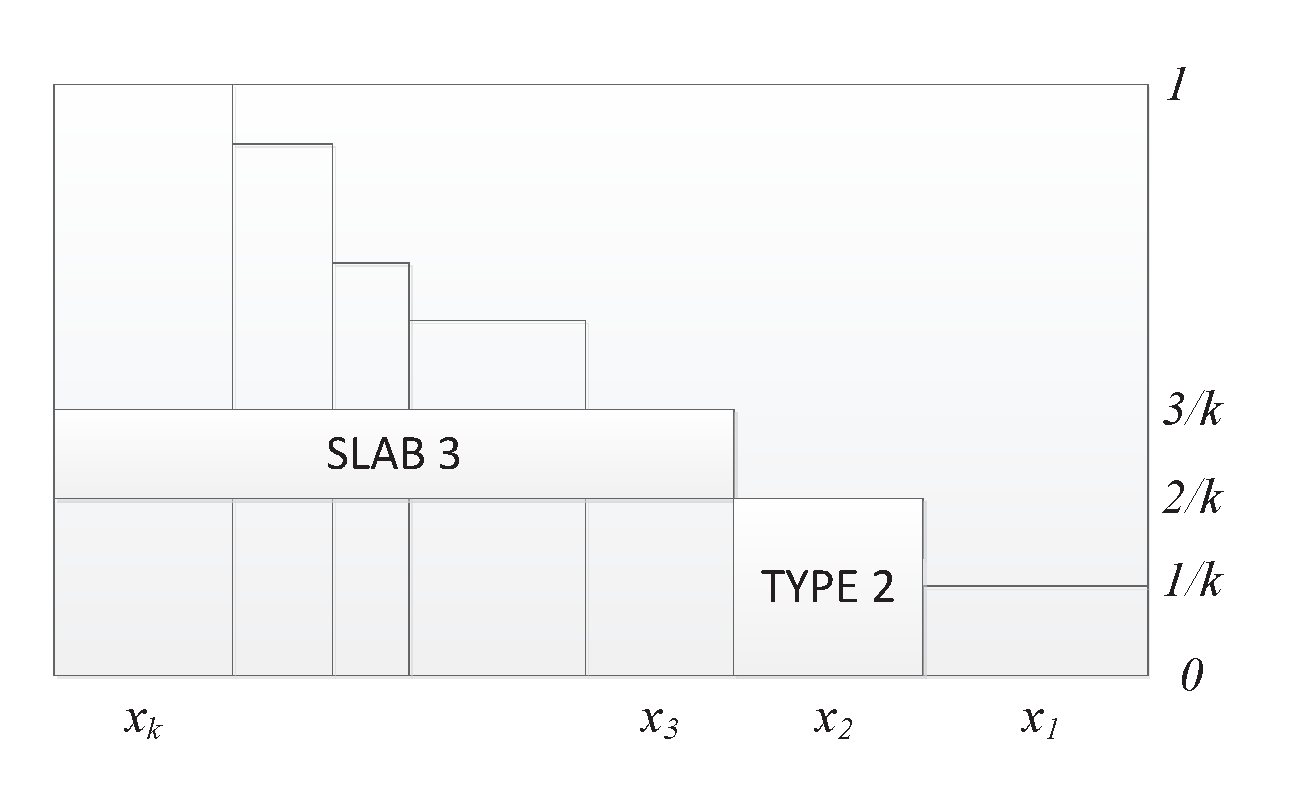
\includegraphics[width=\figwidth]{analysis.eps}\\
    \caption{The APs in each period are ordered from right to left in order of increasing type. We have labeled here the APs in each period of type 2 and the traffic in slab 3.}\label{fig:analysis_amount}
  \end{figure}
  \begin{lemma}
    \begin{equation*}
      \forall\; i,1\leq i\leq k-1:\;\;\;\;\sum_{j=1}^i(1+\frac{i-j}{k})x_j\leq \frac{i}{k}(2n-1)N.
    \end{equation*}
  \end{lemma}

  \begin{IEEEproof}
    From Lemma~\ref{le:type_slab}:
    \begin{eqnarray*}
      \sum_{j=1}^{i}x_j\leq \sum_{j=1}^{i}\beta_j&=&\beta_1+\sum_{j=2}^{i}\beta_j\\
      &=&\frac{i}{k}(2n-1)N-\sum_{j=1}^{i}\frac{i-j}{k}x_j.\\
    \end{eqnarray*}

  \end{IEEEproof}

  The traffic of {\scshape Simplified-Association Algorithm} is
  \begin{eqnarray*}
    \alpha-\rm{AS} &\geq& \sum_{i=1}^{k-1}\frac{i}{k}x_i+[(2n-1)N-\sum_{i=1}^{k-1}x_i]-\frac{(2n-1)N}{k}\\
       & = &(2n-1)N-\sum_{i=1}^{k-1}\frac{k-i}{k}x_i-\frac{(2n-1)N}{k}.
  \end{eqnarray*}

  This gives the following LP, which we call $L$.  In both the constraints below, $i$ ranges from $1$ to $k-1$.
  \begin{eqnarray*}
    \begin{aligned}
        \mbox{max} & \;\;\;\; \Phi=\sum_{i=1}^{k-1}\frac{k-i}{k}x_i, \\
        \mbox{subject to}& \;\;\;\;
        \begin{aligned}
          \forall i: \;\; & \sum_{j=1}^{i}(1+\frac{i-j}{k})x_j\leq \frac{i}{k}(2n-1)N\\
          \forall i: \;\; & x_i\geq 0.
        \end{aligned}
    \end{aligned}
  \end{eqnarray*}
  And the dual LP, $D$, will be used in the case of arbitrary demand bandwidth.
  \begin{eqnarray*}
    \begin{aligned}
        \mbox{min} & \;\;\;\; \Phi=\sum_{i=1}^{k-1}\frac{i}{k}(2n-1)Ny_i, \\
        \mbox{subject to}& \;\;\;\;
        \begin{aligned}
          \forall i: \;\; & \sum_{j=i}^{k-1}(1+\frac{j-i}{k})y_j\geq \frac{k-i}{k}\\
          \forall i: \;\; & y_i\geq 0.
        \end{aligned}
    \end{aligned}
  \end{eqnarray*}

  According to the analysis in~\cite{Mehta:2007}, the value of $\Phi$ of the programs $L$ and $D$ goes to $(2n-1)N/e$.

  \begin{lemma}
    The competitive ratio of {\scshape Simplified-Association Algorithm} is at least $1-\frac{1}{e}$.
  \end{lemma}
  \begin{IEEEproof}
    Recall the traffic of {\scshape Simplified-Association Algorithm} is at least $(2n-1)N-\Phi-\frac{(2n-1)N}{k}$, hence it tends to $(2n-1)N(1-\frac{1}{e})$. Since OPT is $(2n-1)N$, the competitive ratio is at least $1-\frac{1}{e}$.
  \end{IEEEproof}


  \subsection{A Tradeoff-Revealing Family of LPs for the Association}
  In this section, we show how one can derive the optimal trade-off function between bid and the available traffic.

 Here is how we proceed: For every monotonically decreasing tradeoff function $\psi$ and every instance $\pi$ of the association problem and write a new LP $L(\pi,\psi)$ for our association algorithm .  Of course, once we specify the association algorithm as well as the input instance, the actual associations between STAs and APs are completely determined.  In particular, the number $\alpha_i$ of APs of type $i$ is fixed.  $L(\pi,\psi)$ is the seeming trivial LP obtained by taking the left hand side of each inequality in the factor revealing LP $L$ and substituting $x_i=\alpha_i$ to obtain the right hand side.  Formally:\\
  Recall the LP $L$ from the previous section:
  \begin{equation*}
    \max\;\; \bm{c}\cdot\bm{x} \;\;\;\;s.t.\;\;\bm{Ax}\leq\bm{b}\;\;\;\;\bm{x}\geq 0.
  \end{equation*}
  Let $\bm{\alpha}$ be a $k-1$ dimensional vector whose $i$th component is $\alpha_i$.  Let $\bm{A\alpha}=\bm{l}$.  We denote the following LP by $L(\pi,\psi)$:
  \begin{equation*}
    \max\;\; \bm{c}\cdot\bm{x} \;\;\;\;s.t.\;\;\bm{Ax}\leq\bm{l}\;\;\;\;\bm{x}\geq 0.
  \end{equation*}
  The dual LP is denoted by $D(\pi,\psi)$ and is:
  \begin{equation*}
    \min\;\; \bm{l}\cdot\bm{y} \;\;\;\;s.t.\;\;\bm{A^{T}y}\geq\bm{c}\;\;\;\;\bm{y}\geq 0.
  \end{equation*}

  It is easy to find that the optimal solution for $D$ is also an optimal solution to $D(\pi,\psi)$.  Let $\Delta(\pi,\psi)$ be a $k-1$ dimensional vector whose $i$th component is $(\alpha_1-\beta_1)+\ldots+(\alpha_i-\beta_i)$.  Then $ \bm{l}=\bm{b}+\Delta(\pi,\psi).$

  We are interested in comparing the performance of our association algorithm (abbreviated as ALG) with the optimal algorithm OPT.  The following definitions focus on some relevant parameters comparing how ALG and OPT treat on STA $s$:
  \begin{definition}
    Let $\ALG(s)$ ($\OPT(s)$) denote the traffic piece of STA $s$ divided by the algorithm (OPT).  Say that a traffic piece is of type $i$ if OPT served it by a fractal AP of type $i$, and say that the piece lies in slab $i$ if the algorithm serves it from slab $i$.
  \end{definition}
  \begin{lemma}\label{lemma:6}
    For each STA $s$, each traffic piece such that $1\leq\type(s)\leq k-1$,
    \begin{equation*}
    \OPT(s)\psi(\type(\OPT(s)))\leq \ALG(s)\psi(\slab(\ALG(s))).
    \end{equation*}
  \end{lemma}
  \begin{IEEEproof}
    Consider the arrival of $s$ during the running time of the algorithm.  Since $\type(\OPT(s))\leq k-1$, the AP with whom OPT associated this STA is still actively transmitting the traffic piece $\OPT(s)$ from some slab $j\leq \type(\OPT(s))$ in his period.  The inequality in the lemma follows the criterion used by the algorithm to associate STAs, together with the monotonicity of $\psi$.
  \end{IEEEproof}

  \begin{lemma}
    \begin{equation*}
      \sum_{i=1}^{k-1}\psi(i)(\alpha_i-\beta_i)\leq 0.
    \end{equation*}
  \end{lemma}
  \begin{IEEEproof}
    We start by observing that for $1\leq i\leq k-1$:
    \begin{eqnarray*}
      \sum_{s:\type(\OPT(s))=i}\OPT(s)&=&\alpha_i\\
      \sum_{s:\slab(\ALG(s))=i}\ALG(s)&=&\beta_i.
    \end{eqnarray*}
    By Lemma~\ref{lemma:6},
    \begin{equation*}
    \begin{split}
      \sum_{s:\type(\OPT(s))\leq k-1}[\OPT&(s)\psi(\type(\OPT(s)))\\
      &-\ALG(s)\psi(\slab(\ALG(s)))]\leq0.
    \end{split}
    \end{equation*}

    Next observe that
    \begin{equation*}
      \begin{split}
      \sum_{s:\type(\OPT(s))=k-1}&\OPT(s)\psi(\type(\OPT(s)))\\
      &=\sum_{i=1}^{k-1}\sum_{s:\type(\OPT(s))=i}\OPT(s)\psi(i)\\
      &=\sum_{i=1}^{k-1}\psi(i)\alpha_i.\\
      \end{split}
    \end{equation*}
    And
    \begin{equation*}
      \begin{split}
      &\sum_{s:\type(\OPT(s))\leq k-1}\ALG(s)\psi(\slab(\ALG(s)))\\
      &\leq\sum_{s:\type(\ALG(s))\leq k-1}\ALG(s)\psi(\slab(\ALG(s)))\\
      &=\sum_{i}^{k-1} \ALG(s)\psi(\slab(i))\\
      &=\sum_{i}^{k-1}\psi(i)\beta_i.
      \end{split}
    \end{equation*}
  \end{IEEEproof}

  \begin{theorem}
    For function $\psi_k$ defined as
    \begin{equation*}
      \psi_k(i):=\sum_{j=i}^{k-1}y_{j}^{*}=1-(1-\frac{1}{k})^{k-i-1},
    \end{equation*}
    the competitive ratio of the algorithm is $(1-\frac{1}{e})$, as $k$ tends to infinity.
  \end{theorem}
  \begin{IEEEproof}
    Let $\bm{y}$ be an optimal solution of $L$. Then the optimal solution to $L(\pi,\psi)$ has value $\bm{l}\cdot\bm{y}^*$.  This equals $(\bm{b}+\Delta)\cdot \bm{y}^*\leq kN/e+\Delta\cdot \bm{y}^*$ (since $ \bm{l}=\bm{b}+\Delta(\pi,\psi).$ and $\bm{b}\cdot \bm{y}^*\leq 2nN/e$).  Now,
    \begin{eqnarray*}
      \Delta\cdot \bm{y}^{*}&=&\sum_{i=1}^{k-1}\bm{y}^{*}((\alpha_1-\beta_1)+\ldots+(\alpha_i-\beta_i))\\
      &=&\sum_{i=1}^{k-1}(\alpha_i-\beta_i)(y_i^{*}+\ldots+y_{k-1}^{*})\\
      &=&\sum_{i=1}^{k-1}(\alpha_i-\beta_i)\psi(i)\\
      &\leq& 0,\\
    \end{eqnarray*}
     hence the competitive ratio of our association algorithm is $(1-\frac{1}{e})$.
  \end{IEEEproof}

  \subsection{``Early Leaving'' STAs}

  In this section we show how our association algorithm and analysis can be generalized to the situation where $s\in S_a$ may disconnect from AP $a$ before the demanded time has been used out. We call this phenomenon ``early leaving''.

  Because our association algorithm involves an AP's bid for the associating STA and the ratio of allocated traffic on the AP, we can take only these two factors into account when considering whether ``early leaving'' have an impact on our analysis.

  First we consider the AP's bid in case of ``early leaving''. During the association time, we don't know whether the STA will use up its time as it demanded. But our association algorithm will naturally choose the AP that will maximize the actual traffic in case of ``early leaving''. For any AP's bid($b'_s \times t_s$), if  $t_s$ loses its accuracy due to ``early leaving'', we assume that the STA left $t$ units before $t_s$. The reduced amount of traffic by this incident is then $b'_s \times t$. It's easy to see that we can maximize $b'_s$ in order to maximize the actual traffic before $t_s-t$. As we have assumed that the budget for every AP is the same, it's impossible for our algorithm to choose an AP with smaller $b'_s$ when a larger one is possible.

  The other factor is the ratio of allocated traffic on the AP at this moment. At the first sight, this ratio has something to do with demanded time of every STA $s\in S_a$, but it doesn't. As stated above, we can only choose to ignore ``early leaving'' at association, and accept it when it happens. This makes us pretend that STAs $s\in S_a$ are going to leave only at the ``agreed'' time. So to this AP, the amount of allocated traffic, both in the past and in the future, is clear without the need of considering time.

  Having ruled out the interference of ``early leaving'' with the only two factors of our association algorithm, we conclude that our analysis is still valid in this general case.

  \section{Evaluation}\label{sec:evaluation}
  In this section, we test our association algorithm on Matlab\cite{MATLAB} and a real TestBed respectively.  We compare the performance of our algorithm with that of the following ones:
  \begin{itemize}
    \item Strongest Signal First (SSF): The default STA-AP association mechanism in the 802.11 standard.
    \item Largest Available Bandwidth (LAB): The STAs will associate with the APs which has the largest available bandwidth compared with the demanded bandwidth of the STAs based on 802.11e.
  \end{itemize}

  In order to compare our algorithm with other association algorithms in variety of settings, we select several different bandwidth allocation algorithms. The various cases of test algorithms are labeled in Table~\ref{tl:algorithm_combinations}.

  \begin{table}[!ht]
  \centering
  \caption{Algorithm Combinations}\label{tl:algorithm_combinations}
  \begin{tabular}{|c|c|c|}
    \hline
    Label & Bandwidth Allocation & Association Algorithm \\
    \hline
    QoS\_F/ALG & Fixed Bandwidth & ALG\\
    \hline
    QoS\_F/SSF & Fixed Bandwidth & SSF\\
    \hline
    QoS\_F/LAB & Fixed Bandwidth & LAB\\
    \hline
  \end{tabular}

  \end{table}
  This set of algorithms are examined carefully according to the performance metrics listed in the following:
  \begin{itemize}
    \item Per-STA bandwidth in Mbps.
    \item The overall traffic of the network.
    \item The traffic on the APs in Mbps.
    \item The competitive ratio.
  \end{itemize}

  \subsection{Simulations}
  First, we report our simulation results for the scenario where the network contains either static or mobile STAs.  Rather than testing this set of algorithms on a single representative network and load, we choose to define a set of benchmark scenarios, each of which, while somewhat unrealistic, serves to illuminate a different facet of STAs in a WLAN.  STAs of a WLAN are either static or dynamic.

  We first consider a static network, which involves 2 fixed APs in the network, and each has a capacity of 4Mbps.  There are 4 STAs accessing the network successively.  The parameters of the APs and the STAs are shown in Table~\ref{tb:parameter_scenario_1}.  Obviously, the network provides service for STA 4 in ALG, and the other 2 algorithms cannot provide service for STA 4 because of the unwise association decisions for STAs 1, 2 and 3.  And this phenomenon develops because of the property of the on-line algorithm.  The APs and the controller do not know the information of the next STA. The algorithms, SSF and LAB, make greedy association decisions to satisfy the current STAs.  The bandwidth allocated to the STAs is so unreasonable that the APs cannot provide the enough bandwidth for the coming STAs such as STA 4 as shown in Table~\ref{tb:scenario_1}.  And ALG allows STA 4 associate with  AP a to achieve more throughput in the system.

  \begin{table*}
  \centering
  \caption{Parameters of the APs and the STAs in scenario 2}\label{tb:parameter_scenario_1}
    \begin{tabular}{|c|c|c|c|c|c|}
      \hline
      \multirow{2}{*}{STAs} & \multirow{2}{*}{START TIME(s)} & \multirow{2}{*}{END TIME(s)} & \multirow{2}{*}{DEMANDED BANDWIDTH(Mbps)} &\multicolumn{2}{|c|}{MAXIMAL BIT RATE(Mbps)}\\
      \cline{5-6}
       &&&& AP a & AP b\\
      \hline
      1  & 0 & 200 & 1 & 4 & 2 \\
      \hline
      2 & 50 & 200 & 1 & 2.7 & 2\\
      \hline
      3 & 100 & 200 & 2 & 2 & 4\\
      \hline
      4 & 150 & 200 & 2 & 3 & 4\\
      \hline
    \end{tabular}
  \end{table*}

  \begin{table*}[htbp]
  \centering
  \footnotesize
  \caption{Scenario 1: Dynamic STAs.\protect\\ The STA 4 could not associate with any AP in the network in the association algorithms, SSF and LAB }\label{tb:scenario_1}
    \begin{tabular}{|c|c|c|c|c|c|c|c|c|c|}
      \hline
      \multirow{4}{*}{Metrics}&\multirow{4}{*}{Algorithms}&\multicolumn{8}{|c|}{APs}\\
      \cline{3-10}
      &&\multicolumn{4}{|c|}{a(4Mbps)}&\multicolumn{4}{|c|}{b(4Mbps)}\\
      \cline{3-10}
      &&\multicolumn{4}{|c|}{STAs}&\multicolumn{4}{|c|}{STAs}\\
      \cline{3-10}
      &&1&2&3&4&1&2&3&4\\
      \hline
      \multirow{3}{*}{Association}
      &QoS\_F/ALG&$\surd$ &&&$\surd$&&$\surd$&$\surd$&\\
      \cline{2-10}
      &QoS\_F/SSF&$\surd$ &$\surd$&&$\otimes$&&&$\surd$&$\otimes$\\
      \cline{2-10}
      &QoS\_F/LAB&$\surd$ &$\surd$&&$\otimes$&&&$\surd$&$\otimes$\\

      \hline
      \multirow{3}{*}{Traffic}
      &QoS\_F/ALG&0.2&0&0&0.1&0&0.15&0.2&0\\
      \cline{2-10}
      &QoS\_F/SSF&0.2&0.15&0&0&0&0&0.2&0\\
      \cline{2-10}
      ($\times 10^3$ Mb)&QoS\_F/LAB&0.2&0.15&0&0&0&0&0.2&0\\

      \hline
    \end{tabular}

  \end{table*}


  Scenario 2 involves 9 APs and many mobile STAs in a $100\times100m^2$ network.  The locations of the APs are fixed as shown in Fig.~\ref{fig:topology_dynamic}. Each AP has a capacity of $54$Mbps.  The arrival and departure of the STAs are subject to the normal distribution. There are two peak hours, 15 and 21, during a day (24 hours) as shown in Fig.~\ref{fig:traffic_network_request}.  The locations of the STAs are random in the network .  We plot the network traffic under ALG and LAB as shown in Fig.~\ref{fig:traffic_network}.  The network traffic in ALG improves about $37\%$ compared with the LAB algorithm.  And it is obvious that the traffic on each AP under ALG is more balancing compared with LAB as shown in Fig.~\ref{fig:traffic_on_ap_alg} and Fig.~\ref{fig:traffic_on_ap_lab}.

  \begin{figure}[!ht]
    \centering
    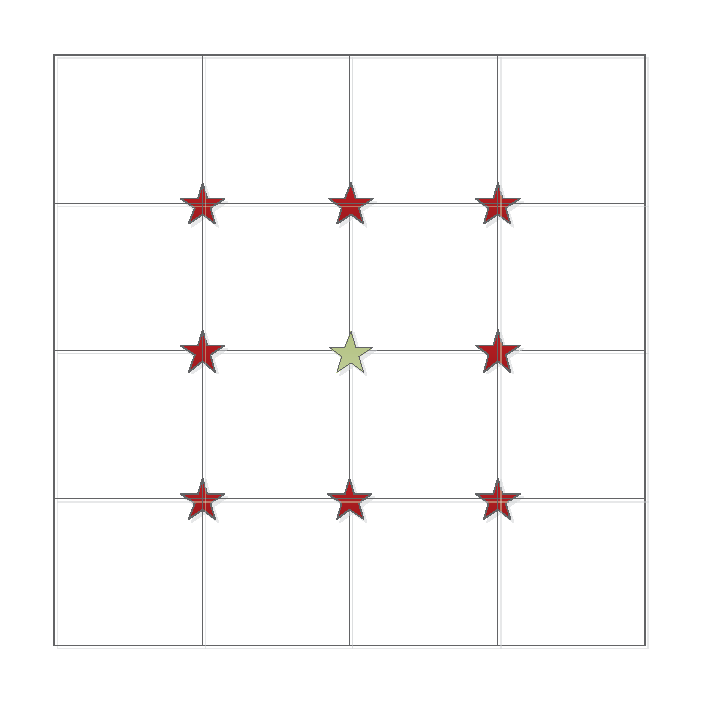
\includegraphics[width=0.3\textwidth]{Topology_Dynamic.eps}\\
    \caption{The topology of the static network}\label{fig:topology_dynamic}
  \end{figure}

  \begin{figure*}[!ht]
  \centering
   \subfigure[Network traffic request of the system]{\label{fig:traffic_network_request}
  \includegraphics[width=\subfigwidth]{Network_Traffic_Requested.eps}}
  \subfigure[Network traffic of the system]{\label{fig:traffic_network}
  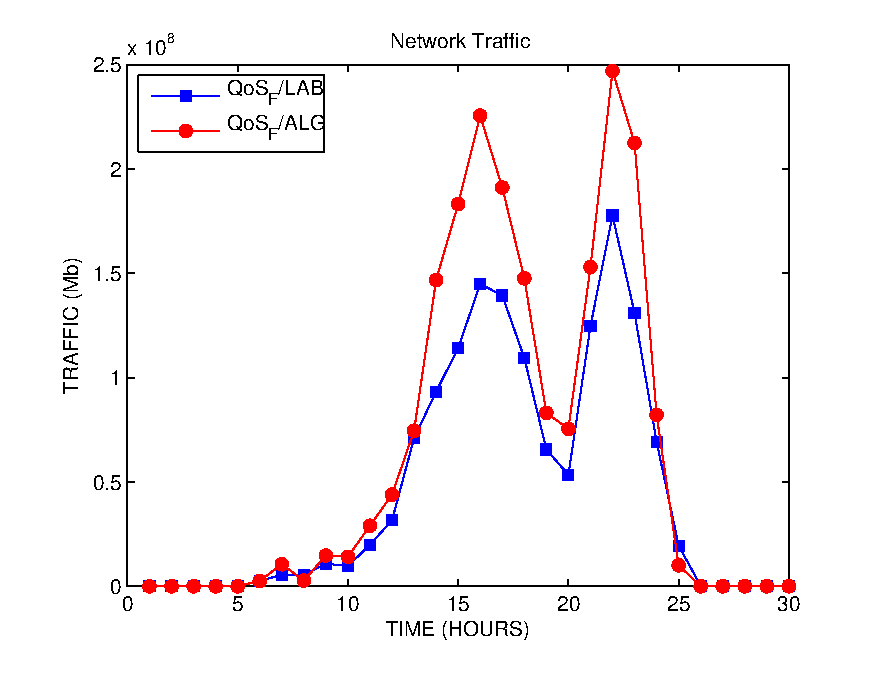
\includegraphics[width=\subfigwidth]{Network_Traffic_Dynamic.eps}}
  \subfigure[Traffic on the APs under ALG]{\label{fig:traffic_on_ap_alg}
  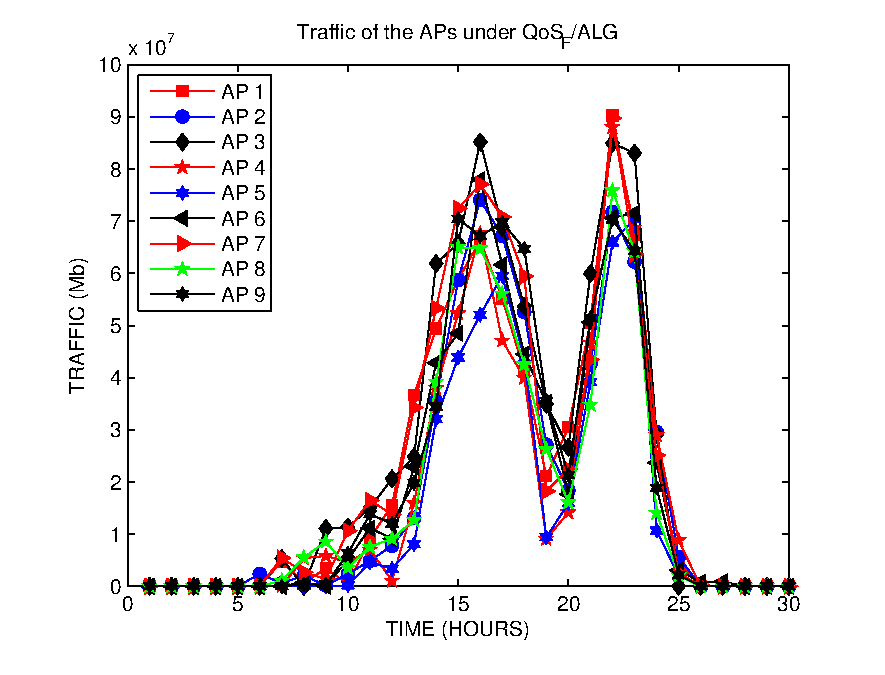
\includegraphics[width=\subfigwidth]{Network_Traffic_AP_ALG.eps}}
  \subfigure[Traffic on the APs under LAB]{\label{fig:traffic_on_ap_lab}
  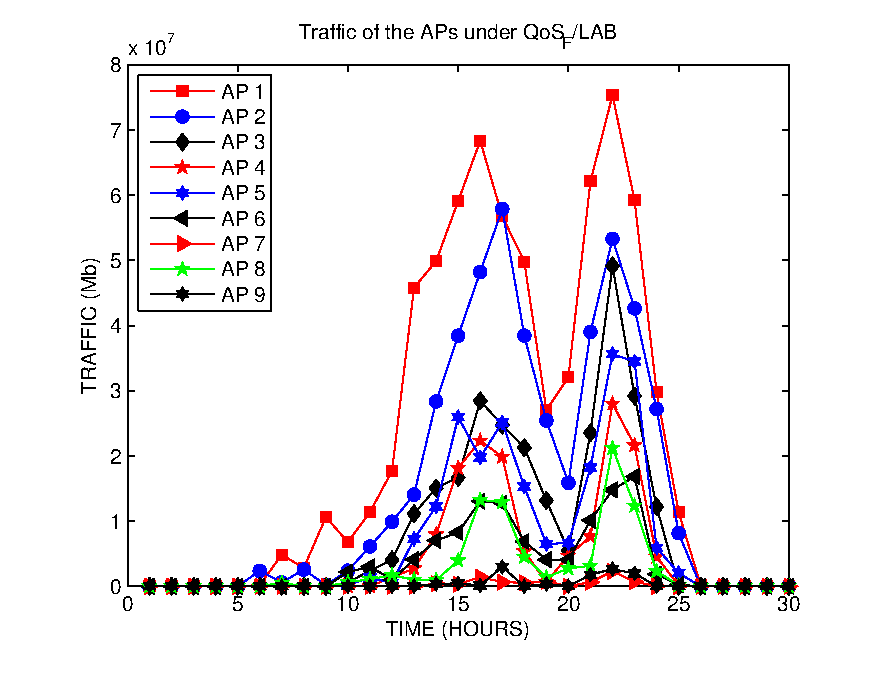
\includegraphics[width=\subfigwidth]{Network_Traffic_AP_LAB.eps}}
  \caption{Scenario 3: Dynamic Network.}\label{fig:scenario_2}
  \end{figure*}

  Scenario 3 involves 3 fixed APs in the network, each has a capacity of 4 Mbps as shown in Fig.~\ref{fig:topology_static}.  And the maximal bit rates between the APs and the STAs are the capacity of the APs.  Then we can get the competitive ratio compared with SSF as shown in \ref{fig:competitive_ratio}.
  \begin{figure}[!ht]
    \centering
    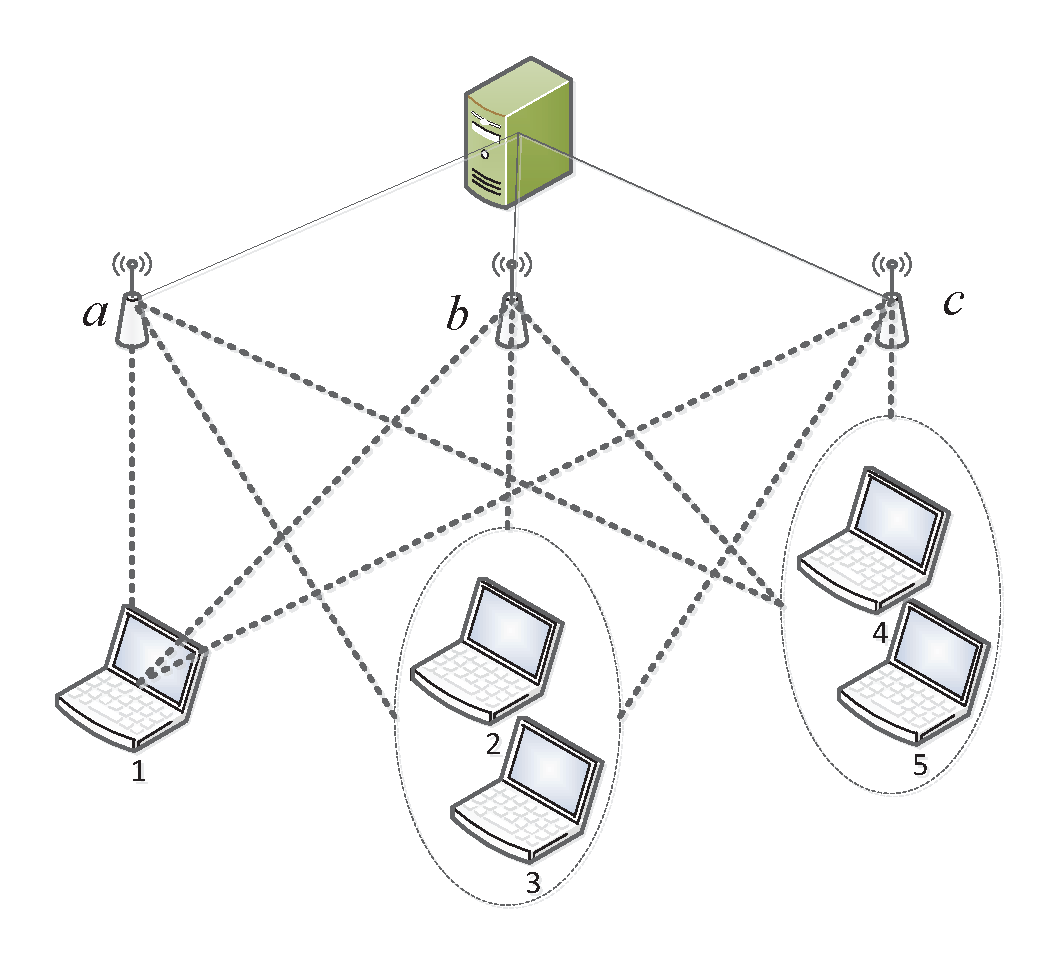
\includegraphics[width=\figwidth]{Topology_Static.eps}\\
    \caption{The topology of the static network}\label{fig:topology_static}
  \end{figure}
  \begin{figure}[!ht]
    \centering
    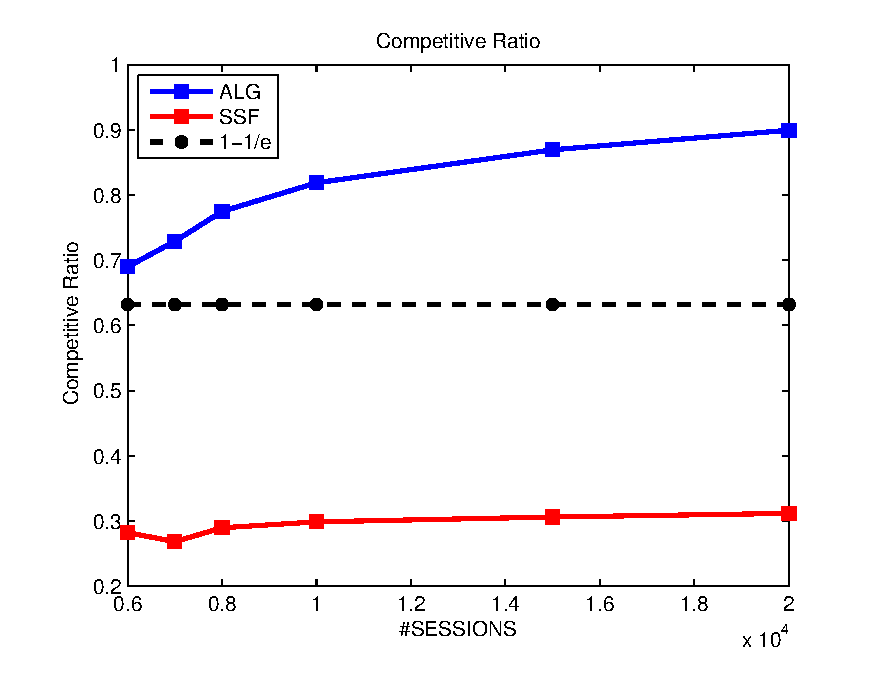
\includegraphics[width=\figwidth]{Competitive_Ratio.eps}\\
    \caption{Competitive Ratio }\label{fig:competitive_ratio}
  \end{figure}

  \subsection{Experiments}

  In this section, we will report our results of experiments which help us understand the performance of our association algorithm.  Experiments are conducted with Thinkpad R61e laptops equipped with Atheros AR2425 802.11g wireless cards.  Each laptop is loaded with the modified Madwifi driver v0.9.4~\cite{madwifi} to collect experimental data.


  The network deploys 2 APs operating in the 802.11g mode on different channels (Channel 11 and Channel 6).  And both APs' maximum bandwidth is 30 Mbps.  There are two stations, STA1 and STA2 associated with AP1 and AP2 respectively.  After a while, STA3 arrives and tries to access the network.  The topology of the network is shown in Fig.~\ref{fig:topology_testbed}.

  In our association algorithm, associations between APs and STAs are launched by AP according to the result of the association algorithm on the controller.  We implemented this function by adding an extra field in the beacon frame set.  STAs will choose APs according to the value in the extra field.  We compare the network traffic of our algorithm with that of LAB and SSF, and present that our algorithm has better performance than the other two as shown in Fig.~\ref{fig:testbed}.  Actually, the network in the testbed is a worse case for our algorithm, because our association algorithm performs better in congested networks. Though this network is light-loaded because of the limited equipment, our algorithm still performs better than the other two.



  \begin{figure}[!ht]
    \centering
    % Requires \usepackage{graphicx}
    \includegraphics[width=\figwidth]{topology_testbed.eps}\\\texttt{\texttt{}}
    \caption{The topology of testbed}\label{fig:topology_testbed}
  \end{figure}

  \begin{figure}
    \centering
    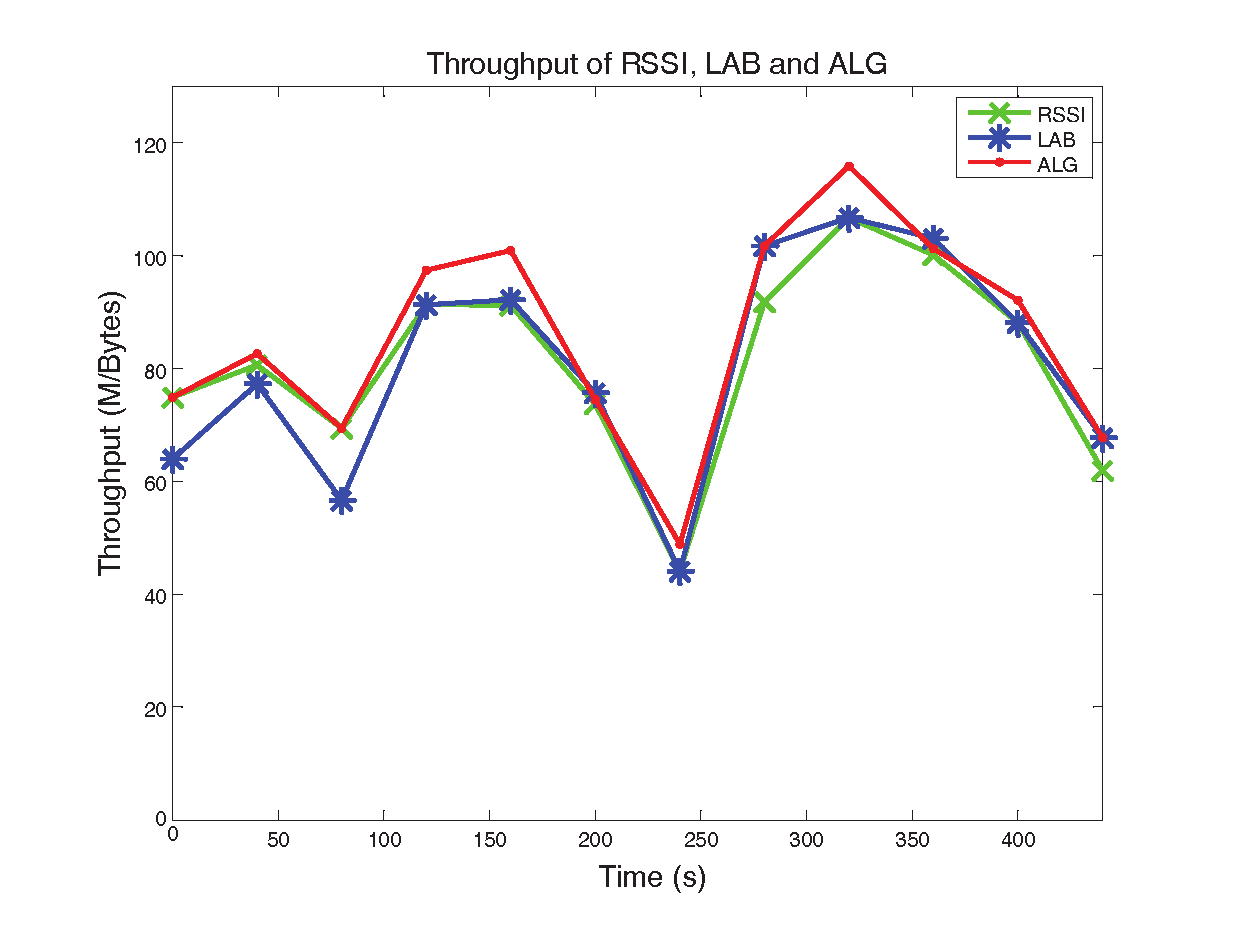
\includegraphics[width=\figwidth]{testbed.eps}\\
    \caption{Scenario 4: The network traffic of the testbed. }\label{fig:testbed}
  \end{figure}

  \subsection{Discussions}\label{sec:discussions}
  In this section we will discuss some practical issues of the implementation of the proposed association algorithm.  According to the states of STAs, the association in our algorithm can be classified into two categories: \textit{Association} and \textit{Reassociation}.  For the \textit{Association}, it is the first time of an STA to associate with an AP.  For the \textit{Reassociation}, the STA has associated with some AP and refreshed its lower bound bandwidth.  Therefore, the STA in the \textit{Association} could not communicate with any AP in the network.  In this case, how does the STA report its demand to the controller by APs?  Actually, the Generic Advertising Service (GAS) in IEEE 802.11u provides the mechanism to communicate with an AP before an STA associates with it.  For the \textit{Reassociation}, how does the AP or controller find the session on the STAs is broken off?  In this situation, the existence of Network Management System (NMS) will the monitor the traffic load on per AP.  When it detects some session has finished or terminated, it will update the information about the associated STAs on the AP.

  \section{Conclusions}\label{sec:conclusion}
  In this paper, we propose a novel on-line association algorithm to deal with any sequence of STAs during a long-term period such as one day.  One important advantage of our algorithm is that it does not need any periodical off-line optimal solutions.  We give a strict proof that the competitive ratio of the algorithm is $1-1/e$ when APs allocate the demanded bandwidth of their associated STAs.  We have extended this property to other feasible bandwidth allocation mechanisms and the bounded-demand STAs.  We evaluate the performance of the algorithm by simulations and experiments in our testbed.  Simulation results show that the proposed association algorithm can improve the network traffic by more than $37\%$ when compared with conventional association algorithms.Our algorithm also performs better than SSF and LAB in the experiments even in a less congested network, which may improve more performance for other association algorithms than that of ours.

  We plan to test and verify the performance of our association algorithm with more APs and more STAs in our testbed. In this condition, we try to find the difference between this experiment and the previous one to optimize our association algorithm. Meanwhile, interference which will influence the performance in a congested network will be taken into consideration in our model.
\section*{Acknowledgment}

This work is supported by Natural Science Foundation of China under Grants No. 61070181, No. 61272524 and No. 61202442.

  \bibliographystyle{IEEETran}
  \bibliography{IEEEabrv,infocom14}






% conference papers do not normally have an appendix


% use section* for acknowledgement





% that's all folks
\end{document}


